\chapter{Multiple Instance Learning}
\section{Fundamentals}
The term multiple instance learning originates from \cite{MILfirstly} and in \cite{mandlik}, the authors proposed the following nomenclature for MIL, which will be reviewed and will be used gladly in our work. 

In standard machine learning problems, each sample is represented by a fixed vector $\boldsymbol{x}$ of observations, however, in multiple instance learning (MIL) it is dealt with samples which are represented by a set of vectors. These vectors are called \emph{instances} and come from an instance space $\pazocal{X}$, for example $\mathbb{R}^D$. The sets of these instances are called \emph{bags} and come from the bag space $\pazocal{B} = \pazocal{P}_F\left(\pazocal{X}\right)$, where $\pazocal{P}_F\left(\pazocal{X}\right)$ denotes all finite subsets of $\pazocal{X}$. With this in mind, we can easily write any bag as $b = \left\lbrace \boldsymbol{x} \in  \pazocal{X} \right\rbrace_{\boldsymbol{x} \in b}$. Each bag $b$ can be arbitrarily large or empty, thus the size of the bag is defined in the form $\vert b\vert \in \mathbb{N}_0$. There may exist intrinsic labeling of instances, but we are only interested in labeling at the bag levels. Bag labels come from a finite set $\pazocal{C}$, and what we want in MIL is to learn a predictor in the form $f_{\boldsymbol{\theta}}: \pazocal{B}\left(\pazocal{X}\right) \rightarrow \pazocal{C}$ that can also be rewritten in the form $f_{\boldsymbol{\theta}}\left(\left\lbrace \boldsymbol{x}\right\rbrace_{\boldsymbol{x}\in b}\right)$. Unlike ML, where a predictor is learned in the form $f_{\boldsymbol{\theta}}:~\mathbb{R}^D~\rightarrow~\pazocal{C}$.  We consider the supervised setting in which each sample of the data set is assigned a label. We can denote the available data by the notation 
\begin{equation}
\pazocal{D}^\star = \Big\lbrace \left(b_i, y_i\right) \in \pazocal{B}\times\pazocal{C} \ | \ i \in \big\lbrace 1,2,\dots,\vert \pazocal{D}^\star \vert \big\rbrace \Big\rbrace, 
\end{equation}
where $\vert \pazocal{D}^\star \vert$ apparently denotes the size of $\pazocal{D}^\star$. The difference between standard ML and MIL is visualized graphically in Figure \ref{MILvsML}.
\begin{figure}[h]
	\centering
	\subfloat[Standard machine learning]
	{{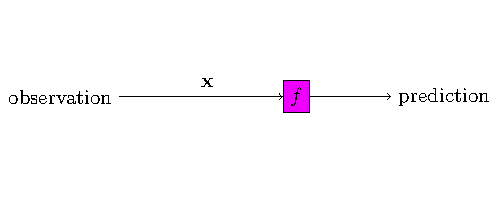
\includegraphics[width=8.0cm]{plots/Images/tikzit_image1} }}%
	\subfloat[Multiple instance learning]
	{{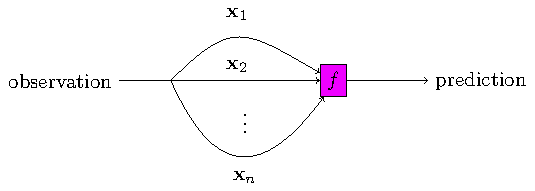
\includegraphics[width=8.0cm]{plots/Images/tikzit_image3} }}%
	\caption{The difference between standard ML and MIL \cite{mandlik}. Standard ML is special case of MIL with $\vert b \vert = 1$. }%
	\label{MILvsML}%
\end{figure}
\section{Embedded-space paradigm}
Very elegant solution to deal with samples on the level bags provides an embedded--space paradigm\cite{mandlik}. This paradigm defines a vector space for the representation of bags and specifies a mapping from each bag $b\in \pazocal{B}$ to this space. Assume that the target vector space is $\R^D$, then the partial mapping $\phi_i$: $\pazocal{B} \to \R,~~ i\in\left\lbrace1,2\dots, D\right\rbrace$~~is defined and overall embedding $\boldsymbol{\phi}: \pazocal{B} \to \R^D $ is given by
\begin{align}
	\boldsymbol{\phi}(b) &= \left(\phi_1(b), \phi_2(b), \dots, \phi_D(b)\right)\\
	&= \left(\phi_1\left(\left\lbrace \bx \right\rbrace_{\bx \in b}\right), \phi_2\left(\left\lbrace \bx \right\rbrace_{\bx \in b}\right), \dots, \phi_D\left(\left\lbrace \bx \right\rbrace_{\bx \in b}\right)\right).
\end{align}
Mappings $\phi_i$ are instrumental in obtaining and aggregating the appropriate information on the level of instances. They can be defined by some instance transformation $k:\pazocal{X}\to \R^D$ and an aggregation function $g:\pazocal{P}_F\left(\R^D\right) \to \R^D$ of the form 
\begin{equation}
	\phi_i(b)=g\left( k\left\lbrace\boldsymbol{x}\right\rbrace_{\boldsymbol{x} \in b}\right).
\end{equation}
On the resulting embedded representation of bag samples, any standard machine learning algorithm can be applied, that is, training a bag-level classifier $f_{\boldsymbol{\theta}}^B :\R^D \to \pazocal{C}$ using an adjusted dataset $\pazocal{D}^\star_{\mathrm{ES}}~=~\Big\lbrace \left(\boldsymbol{\phi}(b_i), y_i\right)~\in~\R^D\times\pazocal{C}~\ ~|~\ i~\in~\big\lbrace 1,2,\dots,\vert D\vert\big\rbrace\Big\rbrace$. The most widely used aggregation functions are minimum, maximum, or mean value
\begin{equation}
    g\left(\left\lbrace x_1,x_2,\dots,x_D \right\rbrace \right) = \begin{cases}
	 \min \left\lbrace x_1,x_2,\dots,x_D\right\rbrace\\
	 \max  \left\lbrace x_1,x_2,\dots,x_D\right\rbrace\\
	 \frac{1}{D}\sum_{i=1}^D x_i \\
\end{cases}   
\end{equation}
\section{Training}\label{MILtraining}
Authors of \cite{mandlik} proposed a versatile unified framework called HMill (Hierarchical multi--instance learning library) for the definition and training of the models and even implemented this functionality in the \emph{Julia} programming language. Furthermore, the framework was published as an open-source project entitled \emph{Mill.jl} under the MIT license. The aim of this work is not to rigorously derive the MIL model, since it is fairly complicated and requires a considerable amount of work. Taking into account that we settled for the MIL model being a neural network (NN) that utilizes aggregation functions on the level of instances and refer to \cite{mandlik} for more details on the definition of the model and its composition.   
Learning of the MIL model $f_{\boldsymbol{\theta}}$ is also supervised, a specific case called binary classification, and therefore achieved by minimizing standard cross--entropy 
\begin{equation}\label{crossentropy52}
	\min_{\boldsymbol{\theta}}- \mathbb{E}_{p_{\mathrm{data}}(\boldsymbol{x},y) }\left[\log \frac{\exp\left({f_{\boldsymbol{\theta}}\left(\boldsymbol{x}\right)[y]}\right)}{\sum_{i=1}^C\exp\left({f_{\boldsymbol{\theta}}\left(\boldsymbol{x}\right)[y_i]}\right)} \right],
\end{equation}   
already mentioned in section \ref{discriminative_modelinmg}. This is very important to us and we will take advantage of that in our experiments.
 
\section{Cross--validation on MIL datasets}\label{experimentCV}
For the MIL testing, we have four datasets available, namely Musk1, Musk2, Tiger and Fox. These datasets are from the UCI database and specially modified for modeling with set data.  All of them will be used to assess the performance of the MIL model.
\subsection{Setup}
In this experiment, data sets are 100 times randomly split into 2 sets in advance, train and test sets, with 80\% of observations being in train set and 20\% of observations belonging to the test set. For future simplification, let a number of random splits be denoted by $r$, and thus $r=100$.  We fit the model on train set, then we evaluate the prediction error on the train data by cross--entropy \ref{crossentropy}. The objective here is to plot the dependence of the prediction error on the complexity of the model. A smaller number of random splits $r$ were tested, but the results obtained were too noisy. For this reason, such a high $r$ was selected, although the experiment became noticeably expensive to compute.    \\

\begin{figure}[h]
	\centering
	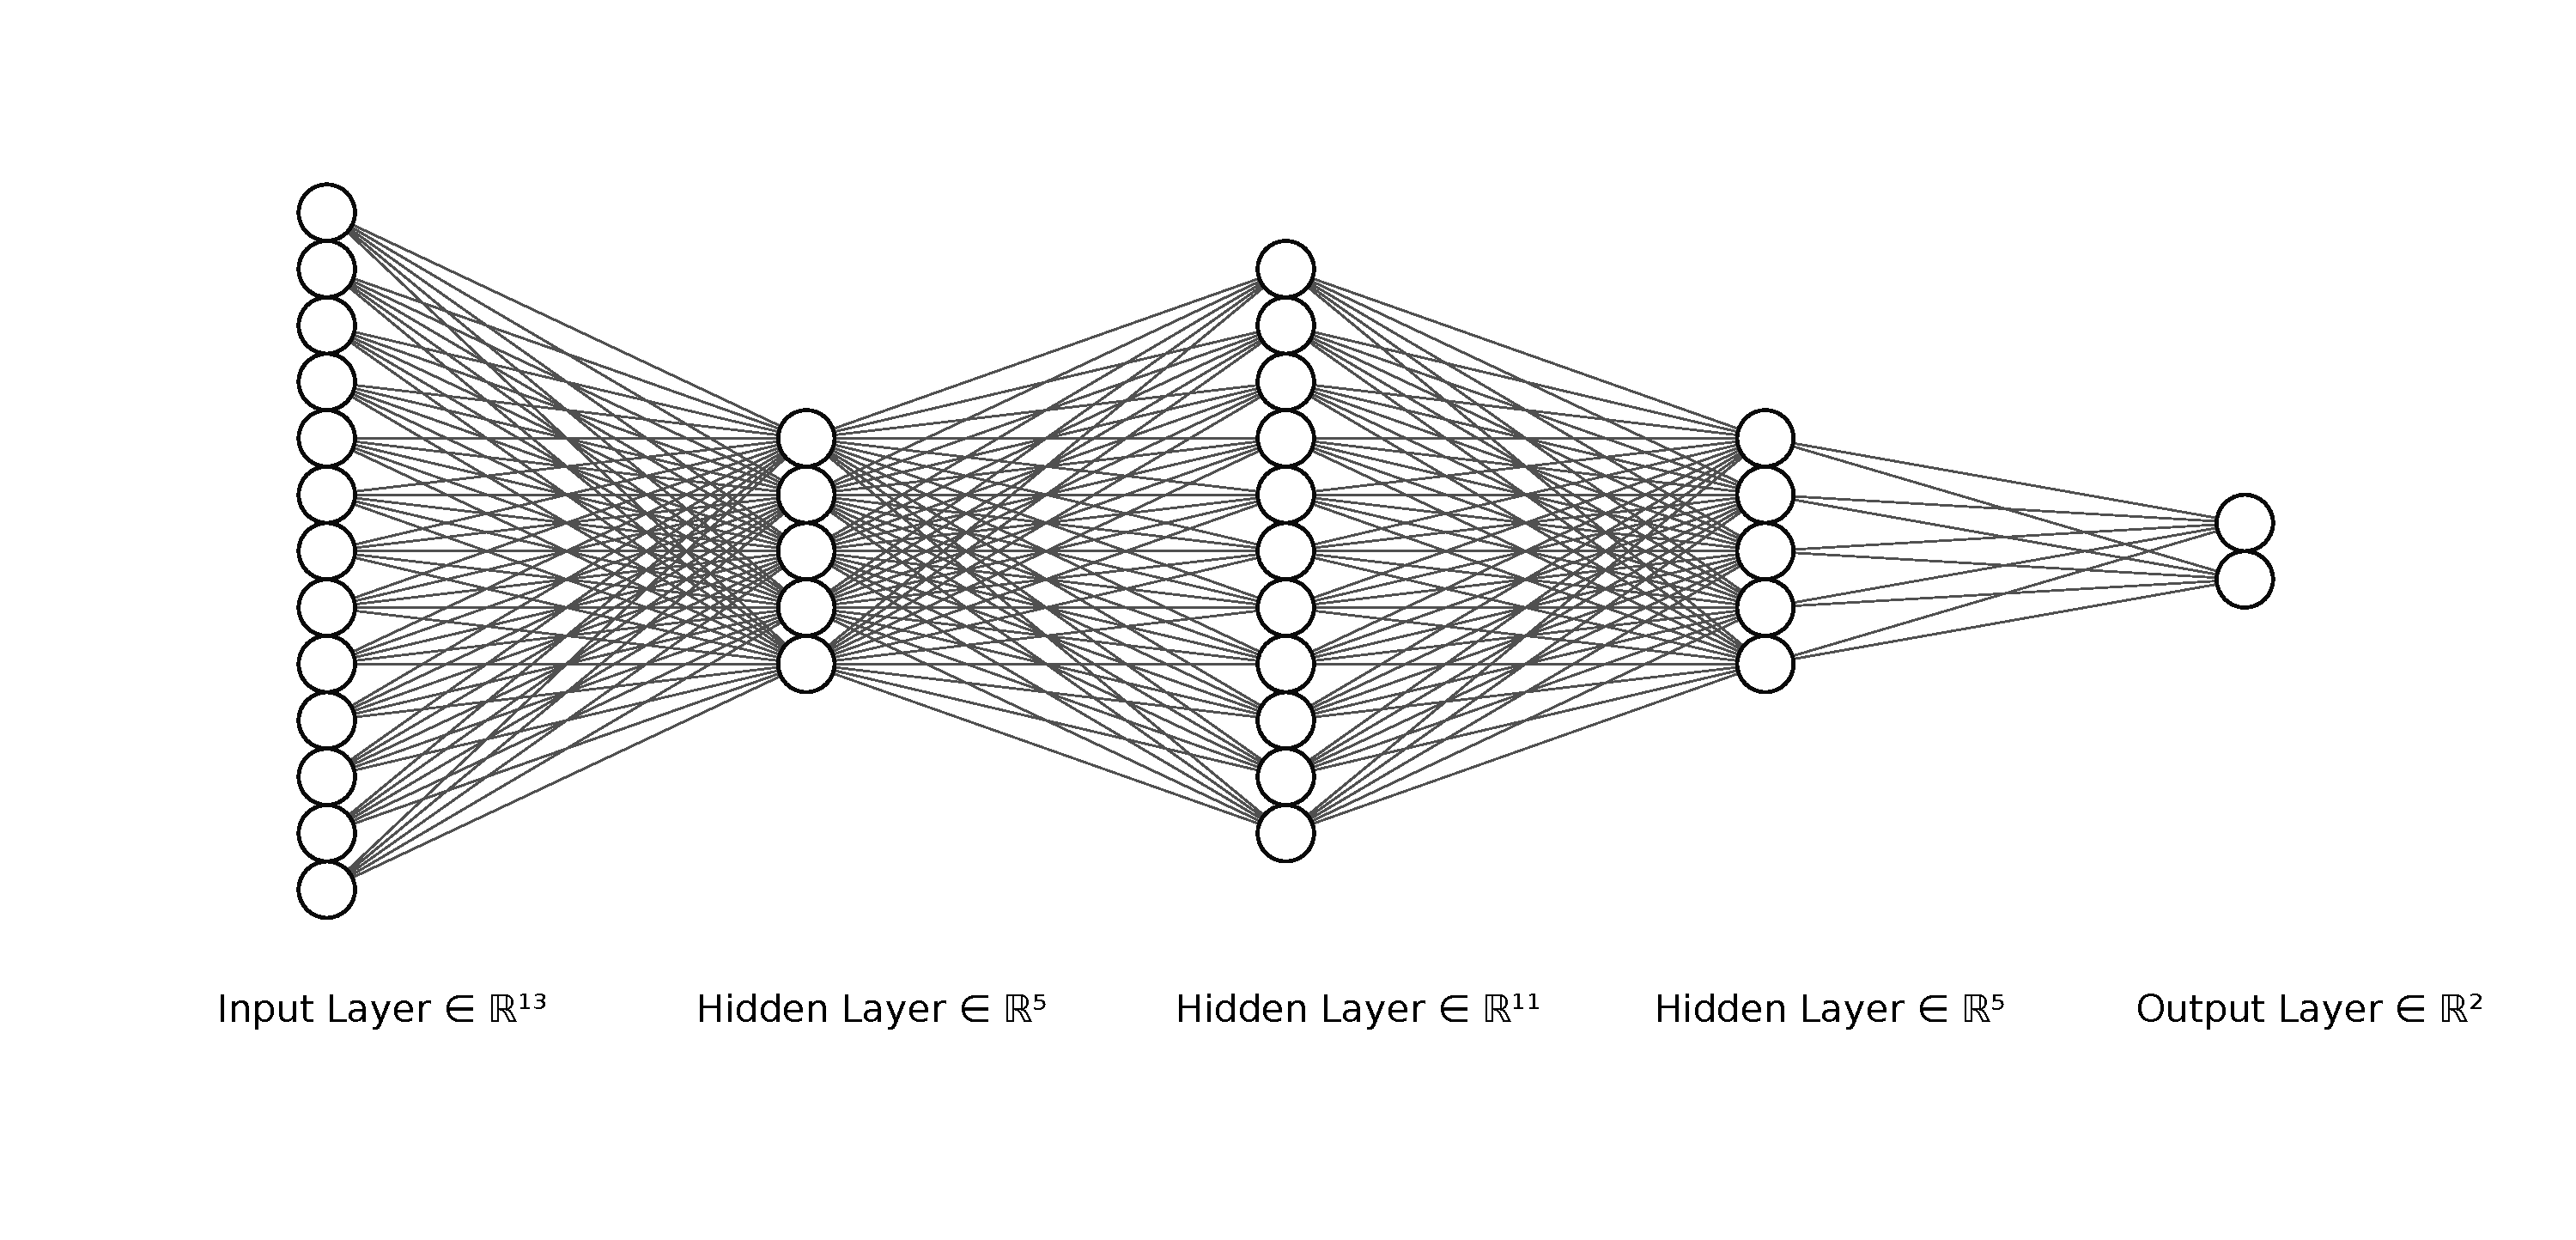
\includegraphics[width=16.0cm, trim={4cm 4.0cm 0.5cm 3.5cm},clip]{plots/Images/nn.pdf}
	\caption{NN example for $z=5$, where input and output layer are only illustrative.}
	\label{NN}
\end{figure}

\begin{para}{Model Complexity}As was mentioned in section \ref{MILtraining}, defining such model for the MIL problem is very complex task, therefore choosing a right model complexity metric is not trivial. Consider a neural network consisting of input layer, 3 hidden layers $h_1\in \R^z, h_2\in \R^{2z+1}, h_3\in \R^z$ and output layer. Then $z \in \left\{1,2,3\dots,20 \right\}$ was selected as model complexity metrics, because this is one of the easiest ways, how to control complexity of the defined MIL model. To gain a better insight, example of such NN is illustrated in Figure \ref{NN}, however this is not the exact NN used in HMill.
\end{para}     

\begin{para}{Prediction Error}
For prediction error metrics, we simply used the standard cross--entropy loss as outlined at the beginning of this section.  There is no need for any trickier objective. Let the total cross--entropy loss evaluated in the $k^{\mathrm{th}}$ random split for fixed $z$ be denoted by $\pazocal{L}_k(z)$, then the estimated prediction error is given by 
\begin{equation}
	\widehat{\mathrm{Err}}(z) = \frac{1}{r}\sum_{k=1}^r \pazocal{L}_k(z).
\end{equation}
\end{para}
\vspace{1cm}

To summarize,  we fit 100 models for selected $z$ on train data and evaluate the prediction error for all of them on test data, then we take the mean value. This process is repeated for each $z~\in~\left\{1,2,3\dots,20 \right\}$, giving 2000 models in total. 
\subsection{Results}
As can be seen in Figure \ref{CV}, the results obtained are totally expected. The prediction error evaluated on the training data for the higher complexity of the model approaches zero. However, testing data give oscillating curves with an increasing trend (with a little exception of Musk1), therefore, model selection is necessary. This applies to each data set.  Furthermore, Table \ref{tab:resultsCV} numerically summarizes the results evaluated in the test data. 

\begin{figure}[h]
	\centering
	\subfloat[CV for dataset Musk1.]
	{{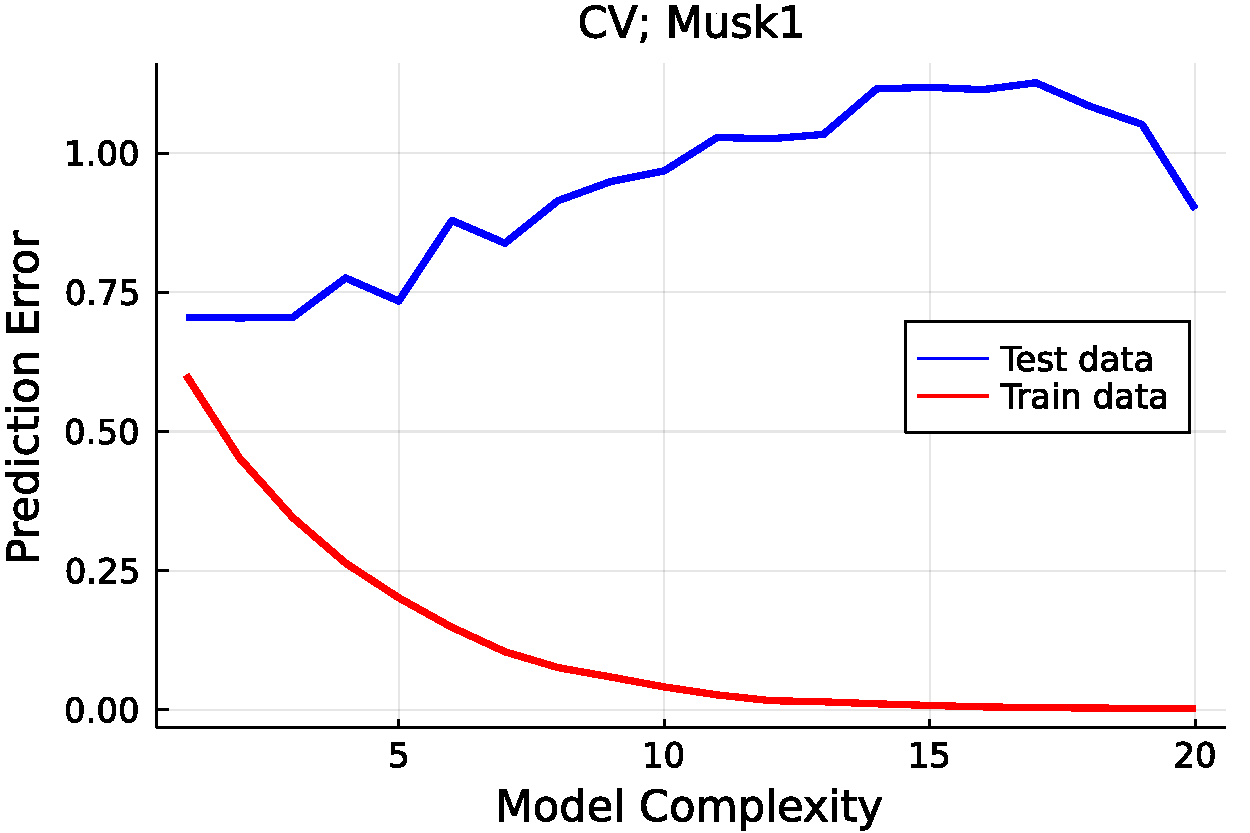
\includegraphics[width=8.0cm]{plots/Images/KFCV_Musk4.pdf} }}%
	\subfloat[CV for dataset Musk2.]
	{{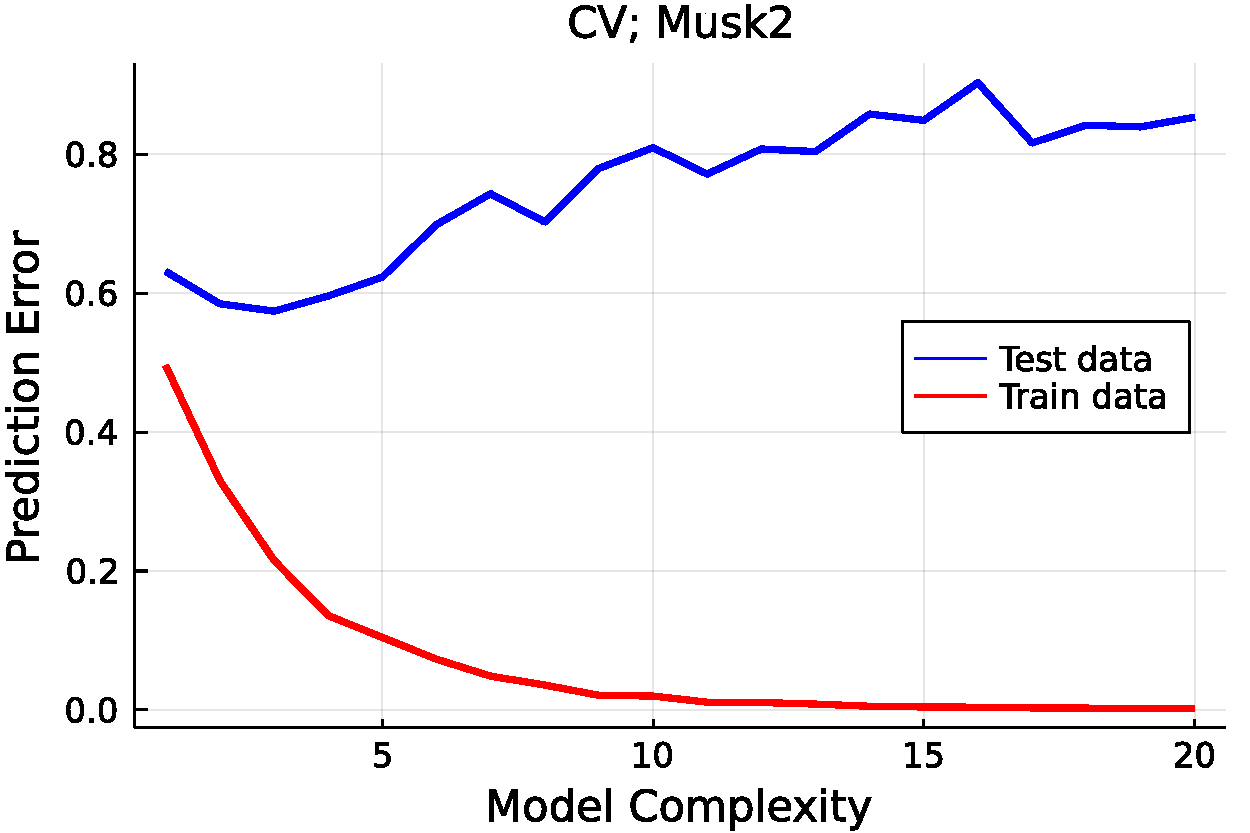
\includegraphics[width=8.0cm]{plots/Images/KFCV_Musk2.pdf} }}%
	\
	\subfloat[CV for dataset Fox.]
	{{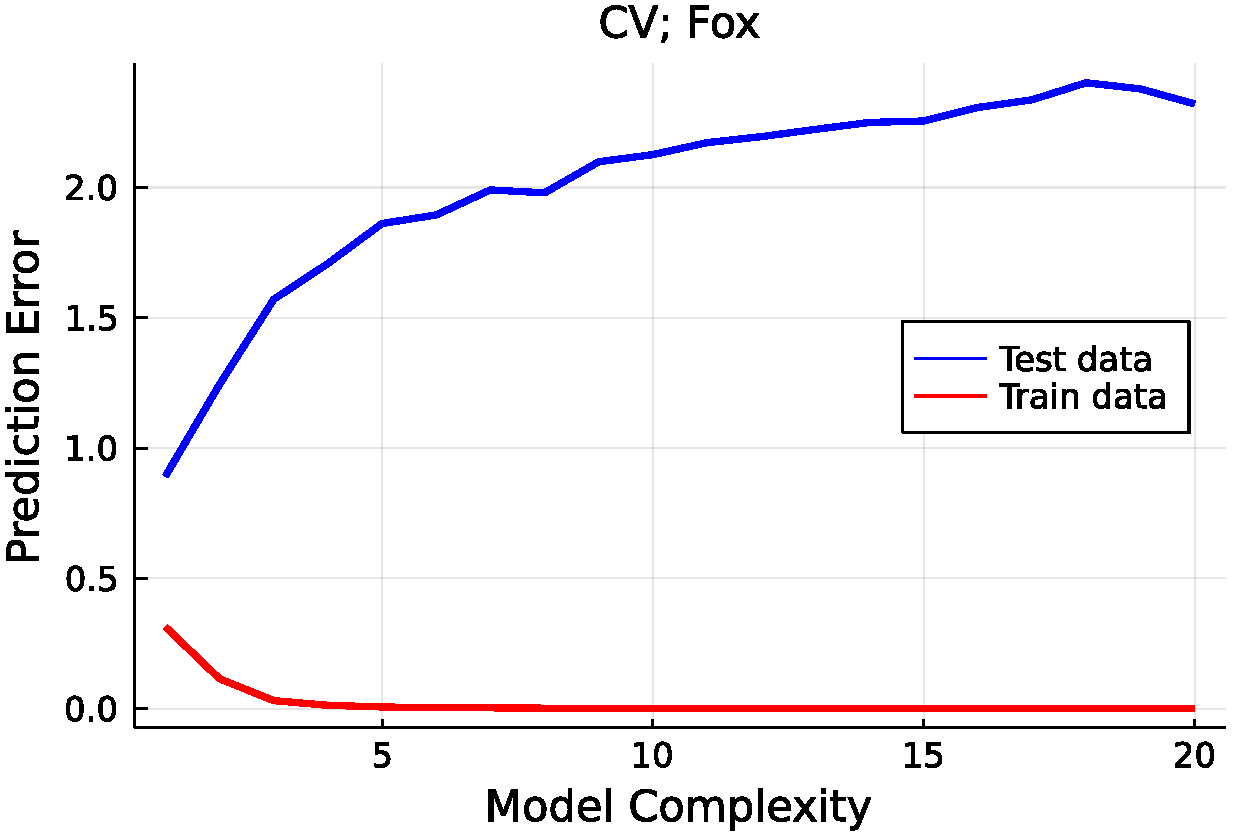
\includegraphics[width=8.0cm]{plots/Images/KFCV_Fox.pdf} }}%
	\subfloat[CV for dataset Tiger.]
	{{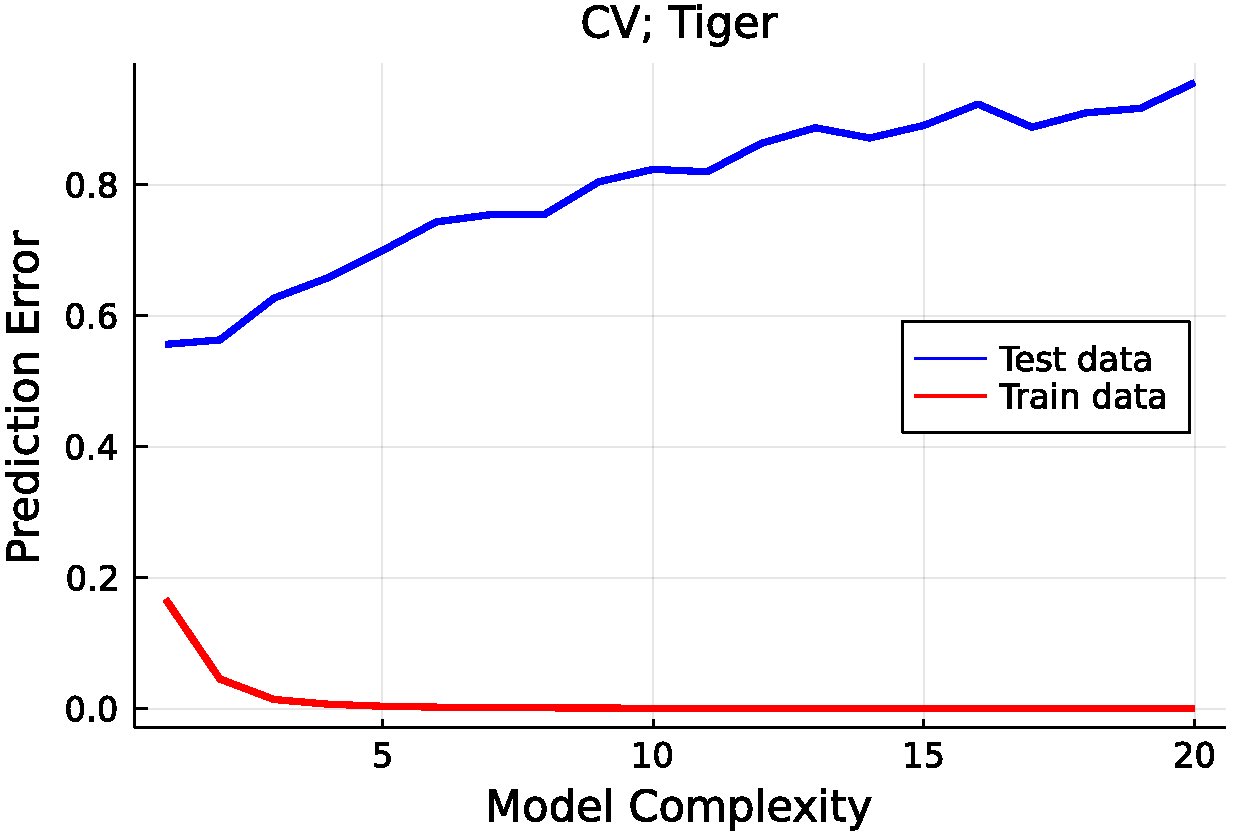
\includegraphics[width=8.0cm]{plots/Images/KFCV_Tiger.pdf} }}%
	\caption{Evaluation of prediction error with the use of training data and testing data on MIL datasets Musk1, Musk2, Fox and Tiger. }%
	\label{CV}%
\end{figure}

\begin{table}[h]
	\centering
	\begin{tabular}{|l|l|l|l|}
		\hline
		Dataset  &$\argmin \widehat{\mathrm{Err}}(z)$ & $ \min \widehat{\mathrm{Err}}(z)$ &$\widehat{\mathrm{Err}}(z=10)$ \\ \hline
		Musk1              & 2        & 0.70& 0.97   \\ \hline
		Musk2              & 3        & 0.57& 0.81   \\ \hline
		Fox               & 1        & 0.89 &  2.13 \\ \hline
		Tiger               & 1        & 0.56  & 0.82    \\ \hline
	\end{tabular}
	\caption{Results of CV evaluated on the testing data.}
	\label{tab:resultsCV}
\end{table}




\section{MIL to HDGM problem}
In the previous part, the CV experiment was performed with the expected results. However, the estimated prediction error seems to be rather high. Logically, the question of whether the prediction error can be reduced has been raised, and also whether it is possible to make $r$ smaller has been raised.
\subsection{Setup}
On the initiative to reduce prediction error, it is proposed to train a MIL model that is obtained by minimizing the hybrid loss function 

\begin{equation}
	\min_{\boldsymbol{\theta}}- \mathbb{E}_{p_{\mathrm{data}}(\boldsymbol{x},y)}\left[\alpha\log \frac{\exp\left({f_{\boldsymbol{\theta}}\left(\boldsymbol{x}\right)[y]}\right)}{\sum_{i=1}^C\exp\left({f_{\boldsymbol{\theta}}\left(\boldsymbol{x}\right)[y_i]}\right)}+ \left(1-\alpha\right)\log \frac{\exp\left({f_{\boldsymbol{\theta}}\left(\boldsymbol{x}_i\right)[y]}\right)}{\sum_{j=1}^N\exp\left({f_{\boldsymbol{\theta}}\left(\boldsymbol{x}_j\right)[y]}\right)} \right].
	\end{equation}
Since the discriminative part is already used in HMill framework, the only task is to add the generative part into it. At this point are available all normalization samples, thus $M=N$. This modification should lead to a reduced prediction error evaluated on training data.\\
In the first part of this experiment, we would like to train models in relation to parameter $\alpha$. For this setup, we need to choose fixed $z$. Since authors of \cite{mandlik} usually use $z=10$, we use this value as well. For the prediction error evaluation is used standard cross--entropy as in the previous experiment, again with $r=100$ and $\alpha \in \left\{0.0, 0.1, 0.2,\dots,1.0\right\}$. Therefore estimated prediction error can be written in the form
\begin{equation}
	\widehat{\mathrm{Err}}(\alpha) = \frac{1}{r}\sum_{k=1}^r \pazocal{L}_k(z=10, \alpha).
\end{equation}
We hope to see a curve in the shape of a bowl that has its global minimum at a point $\alpha=0.5$ or somewhere near.

In the second part, evaluating the prediction error is approached in the other way. The fixed $\alpha = 0.5$ is selected and the dependency on $z~\in~\left\{1,2,3\dots,20 \right\}$ is evaluated as in Section \ref{experimentCV}. Finally, the estimated prediction error in this case is defined by
\begin{equation}
	\widehat{\mathrm{Err}}(z) = \frac{1}{r}\sum_{k=1}^r \pazocal{L}_k(z, \alpha =0.5).
\end{equation}
In other words, the setup is the same as in \ref{experimentCV}, therefore, the results obtained will be added to the figure \ref{CV} and the table \ref{tab:resultsCV} for a convenient comparison. Note that curves for train data from this experiment will be omitted because they are not important at this point. We are only interested in predictions for test data.  
\clearpage
\subsection{Results}



The results of the first part are represented in Figure \ref{fig:HDGE} and Table \ref{tab:resultsHDGE}, where it can be seen that adding the generative term to the MIL loss function decreased the prediction error evaluated on all datasets. This improvement is considerable on datasets Musk1 and Musk2, where a nice bowl can be seen. On Fox and Tiger datasets such an improvement does not occur. This means that HDGM approach works, thus regularization in the form of a very simple generative term may bring improvement in predictions. Unfortunately, the choice of $\alpha=0.5$ was not confirmed as the best in our experiment; see Table \ref{tab:resultsHDGE}.   

In the second part of the experiment, the results are shown in Figure \ref{fig:resultsHDGMz} and Table \ref{tab:HDGMz}. Here is a situation very similar to the previous part of this experiment. Improvement of the prediction error is quite noticeable on the first two datasets Musk1 and Musk2, while Fox and Tiger do not look so convincingly. Furthermore, the number of random splits $r=100$ is still needed to remove the noise from the prediction error. 

In general, it can be said that the HDGM approach leads to a small decrease in the prediction error. 
\begin{table}[h]
	\centering
	\begin{tabular}{|l|l|l|l|}
		\hline
		Dataset  &  $\argmin \widehat{\mathrm{Err}}(\alpha)$& $\min \widehat{\mathrm{Err}}(\alpha)$ \\ \hline
		Musk1              & 0.4      & 0.68   \\ \hline
		Musk2             & 0.2      & 0.54   \\ \hline
		Fox                 & 0.7      & 1.89  \\ \hline
		Tiger            & 0.4      & 0.74      \\ \hline
	\end{tabular}
	\caption{Prediction error statistics for HDGM in case of $z=10$.}
	\label{tab:resultsHDGE}
\end{table}
\begin{figure}[h]
	\centering
	\subfloat[HDGM for dataset Musk1.]
	{{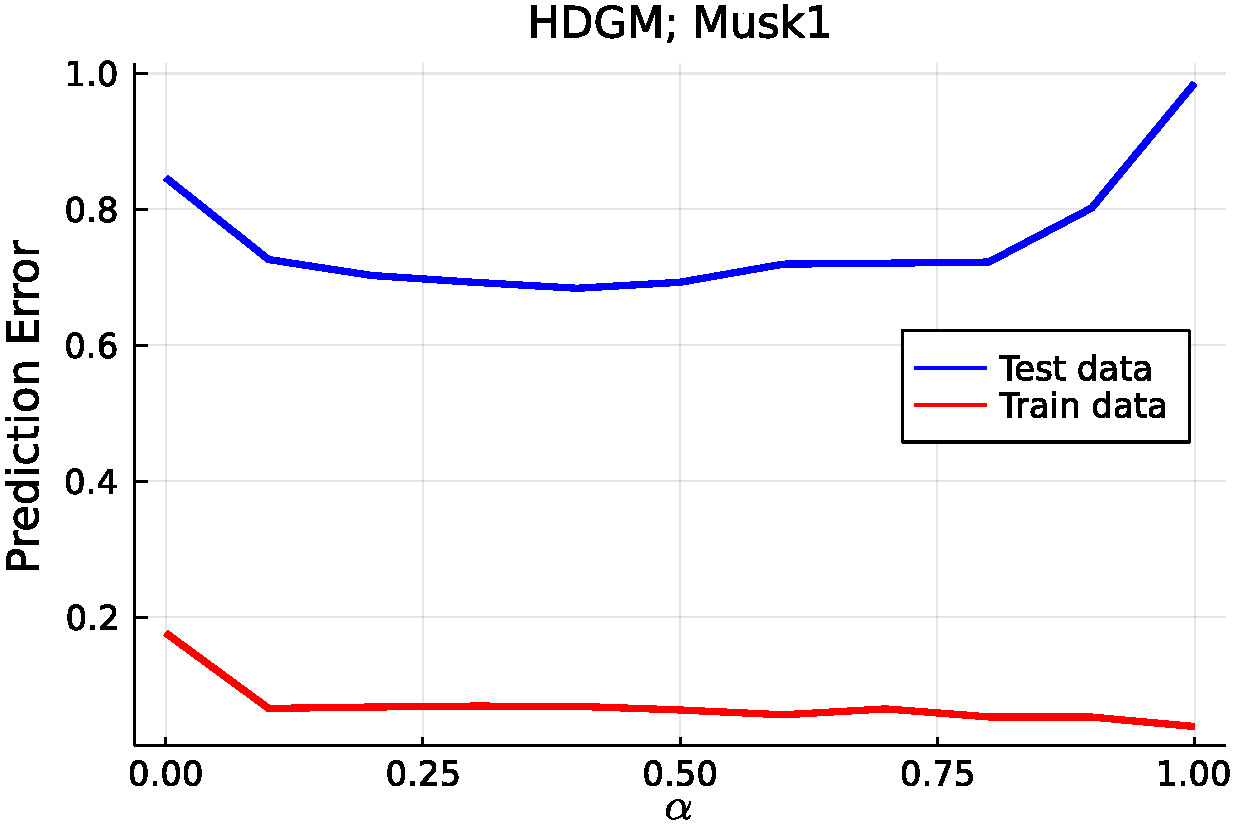
\includegraphics[width=8.2cm]{plots/Images/HDGM_Musk3.pdf} }}%
	\subfloat[HDGM for dataset Musk2.]
	{{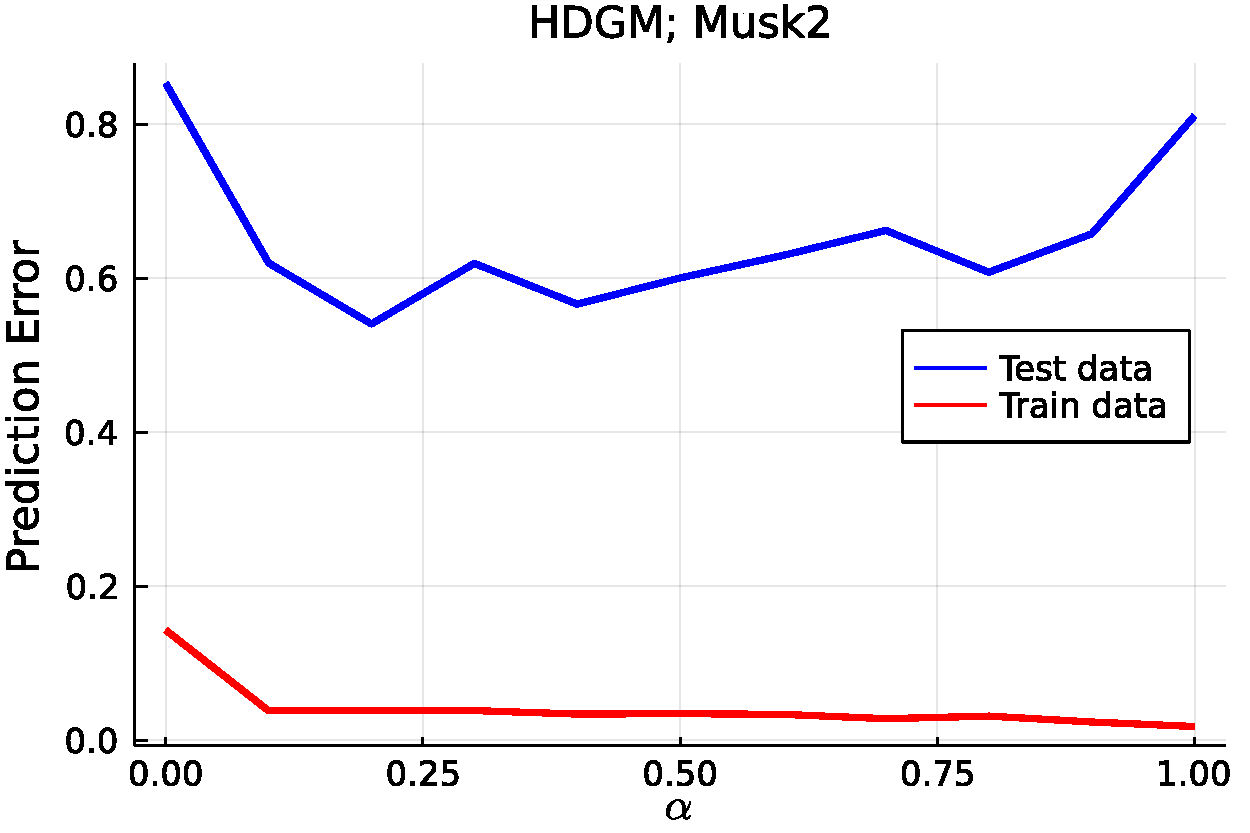
\includegraphics[width=8.2cm]{plots/Images/HDGM_Musk4.pdf} }}%
	\
	\subfloat[HDGM for dataset Fox.]
	{{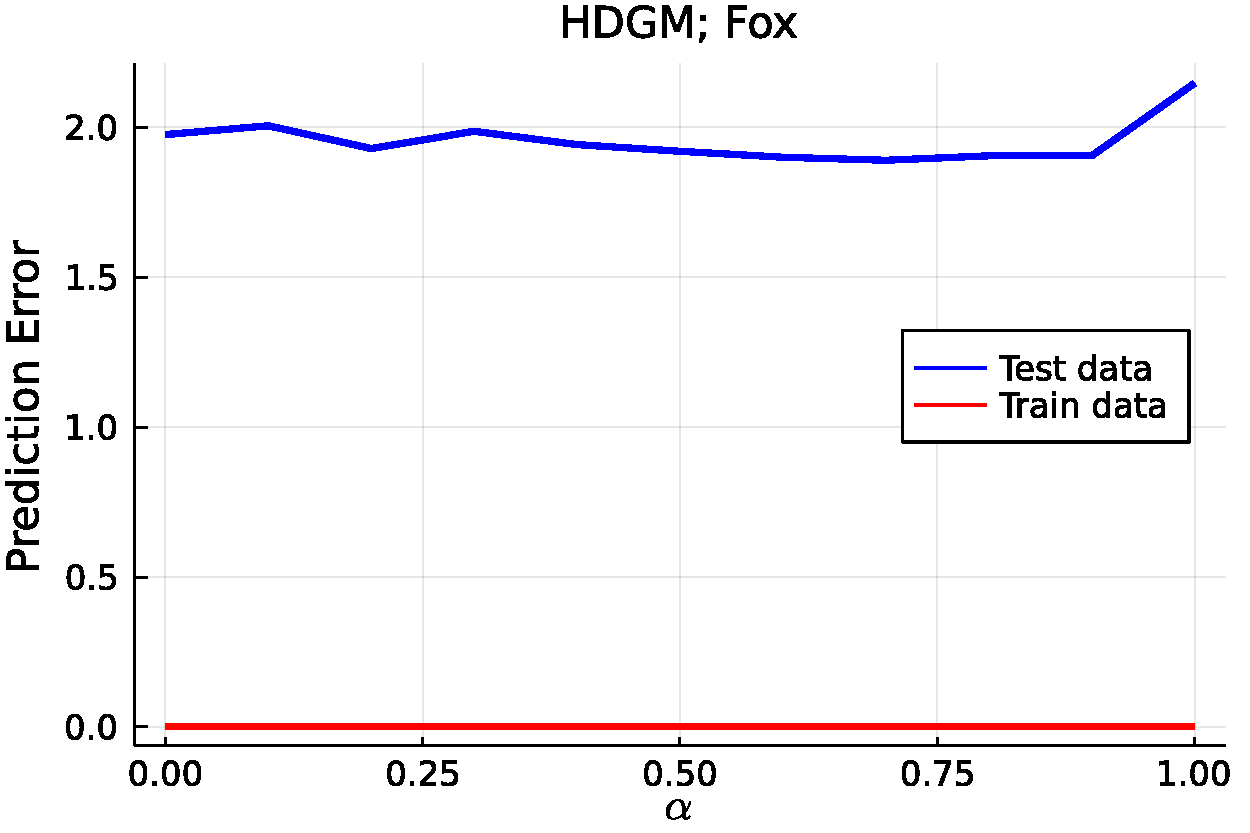
\includegraphics[width=8.2cm]{plots/Images/HDGM_Fox.pdf} }}%
	\subfloat[HDGM for dataset Tiger.]
	{{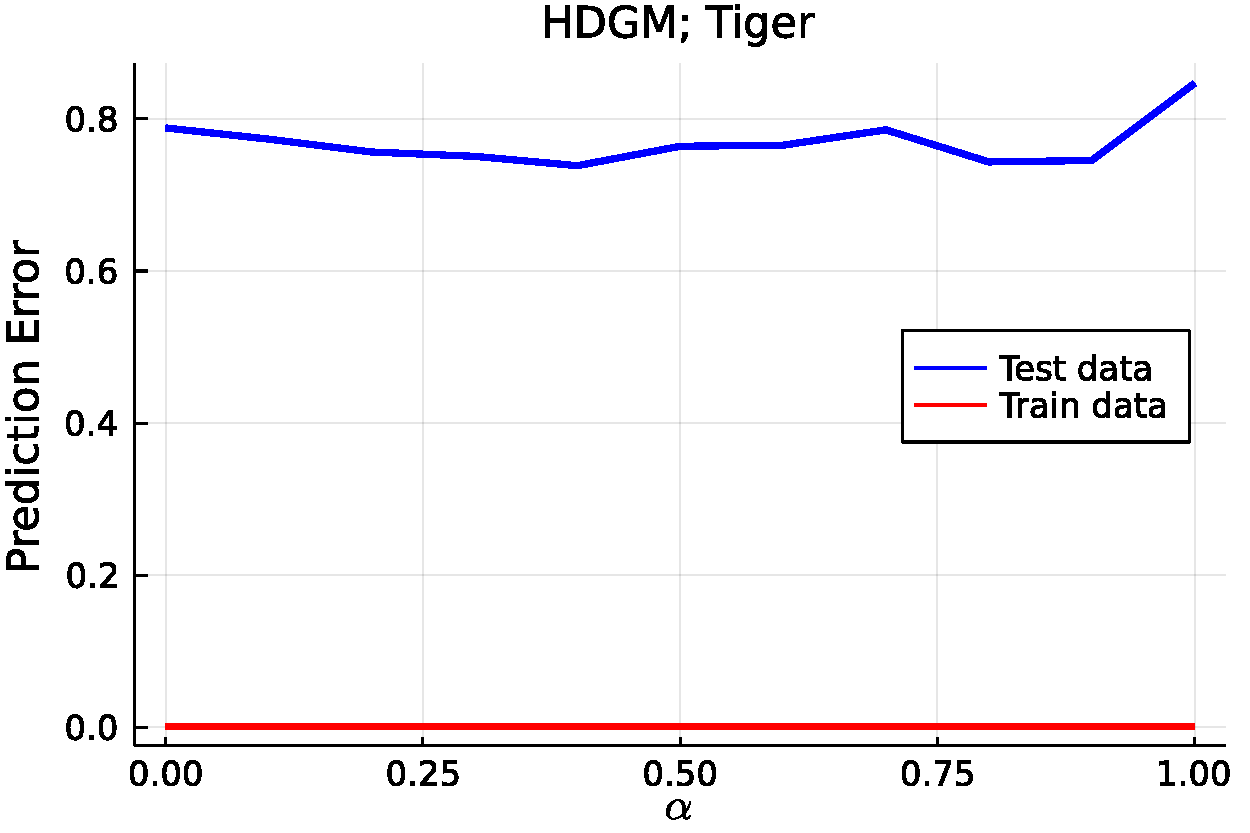
\includegraphics[width=8.2cm]{plots/Images/HDGM_Tiger.pdf} }}
	\caption{Evaluation of the prediction error $\widehat{\mathrm{Err}}(\alpha)$ with the use of training data and testing data on MIL datasets. }%
	\label{fig:HDGE}%
\end{figure}


\begin{table}[h]
	\centering
	\begin{tabular}{|l|l|l|l||l|l|l|}
		\hline
		& \multicolumn{3}{l||}{~~~~~~~~~~~\textbf{Discriminative part only}} & \multicolumn{3}{l|}{~~~~~~~~~~~~~~~~~\textbf{HDGM}; $\alpha=0.5$} \\ \hline
		Dataset & $\argmin \widehat{\mathrm{Err}}(z)$   & $\min \widehat{\mathrm{Err}}(z)$ &$\widehat{\mathrm{Err}}(z=10)$  &   $\argmin \widehat{\mathrm{Err}}(z)$             &     $\min \widehat{\mathrm{Err}}(z)$       &     $\widehat{\mathrm{Err}}(z=10)$         \\ \hline
		Musk1   & 2             & 0.70         & 0.97    &    6          &  0.64           &  \textbf{0.69}           \\ \hline
		Musk2   & 3              & 0.57         & 0.81    &    6          & 0.55            &  \textbf{0.66}           \\ \hline
		Fox     & 1              & 0.89         & 2.13    &    1          &  0.95           &   \textbf{1.96}          \\ \hline
		Tiger   & 1              & 0.56          & 0.82       &   2           &   0.58          &   \textbf{0.80}          \\ \hline
	\end{tabular}
	\caption{Comparison of prediction error statistics for HDGM $\alpha=0.5$ and discriminative part only. Pay attention especially to the last column in each approach, $\widehat{\mathrm{Err}}(z=10)$.}
	\label{tab:HDGMz}
\end{table}

\begin{figure}[h]
	\centering
	\subfloat[HDGM: $\alpha=0.5$ vs Discriminative; Musk1.]
	{{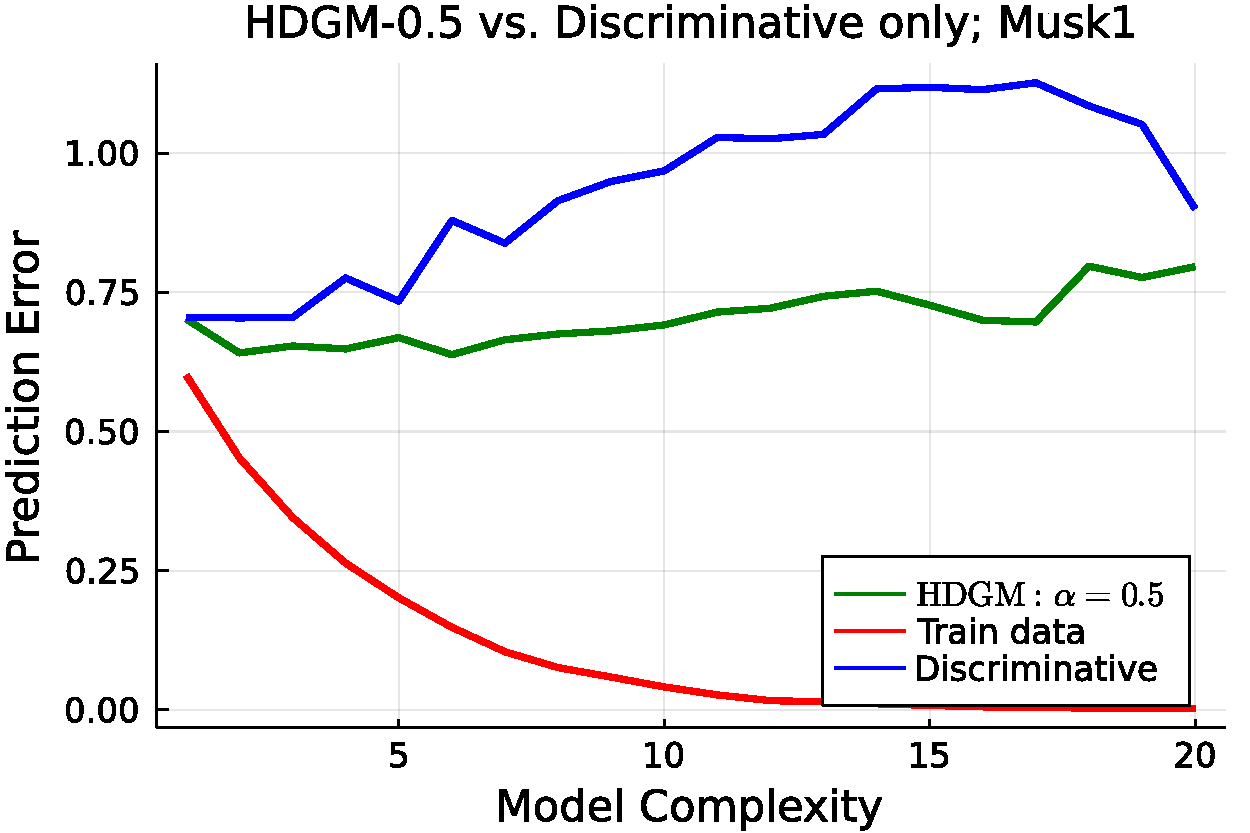
\includegraphics[width=8.2cm]{plots/Images/supervisedvsHDGM0_5_Musk1.pdf} }}%
	\subfloat[HDGM: $\alpha=0.5$ vs Discriminative; Musk2.]
	{{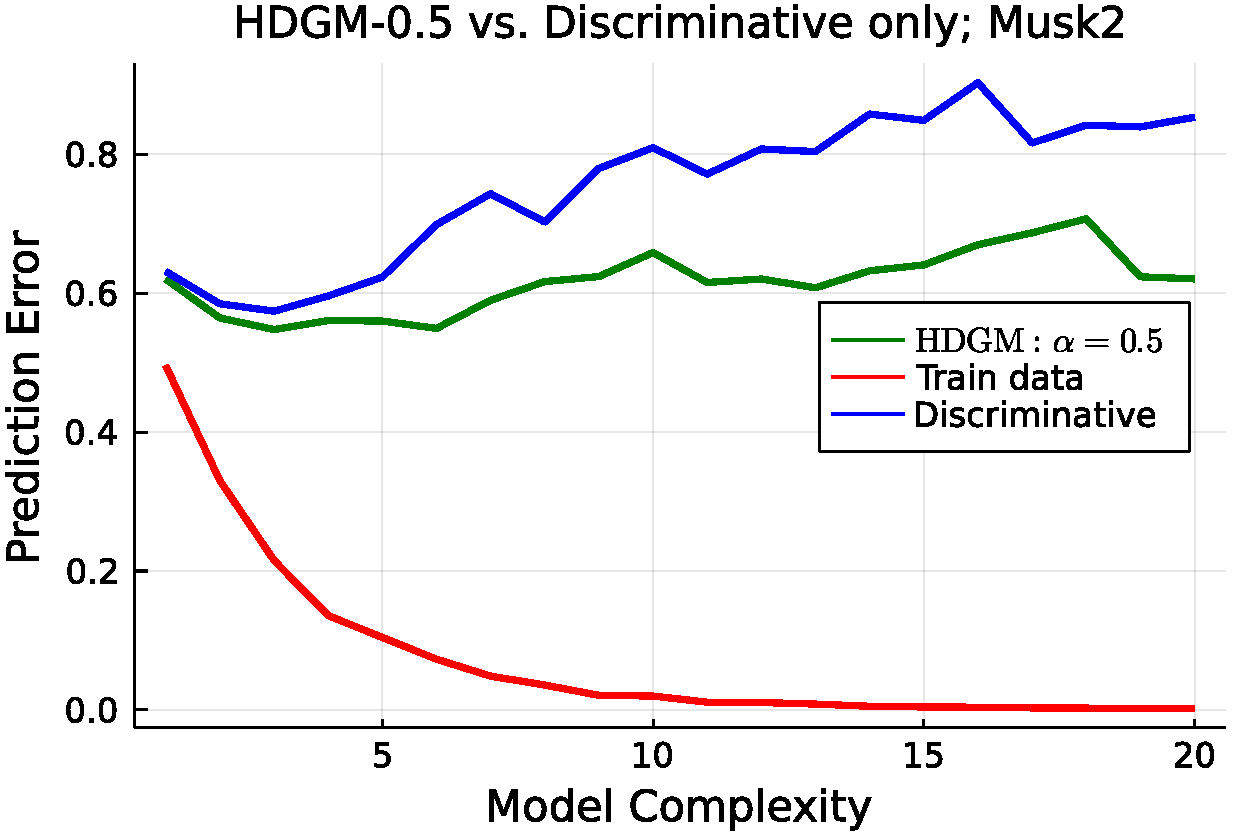
\includegraphics[width=8.2cm]{plots/Images/supervisedvsHDGM0_5_Musk2.pdf} }}%
	\
	\subfloat[HDGM: $\alpha=0.5$ vs Discriminative; Fox.]
	{{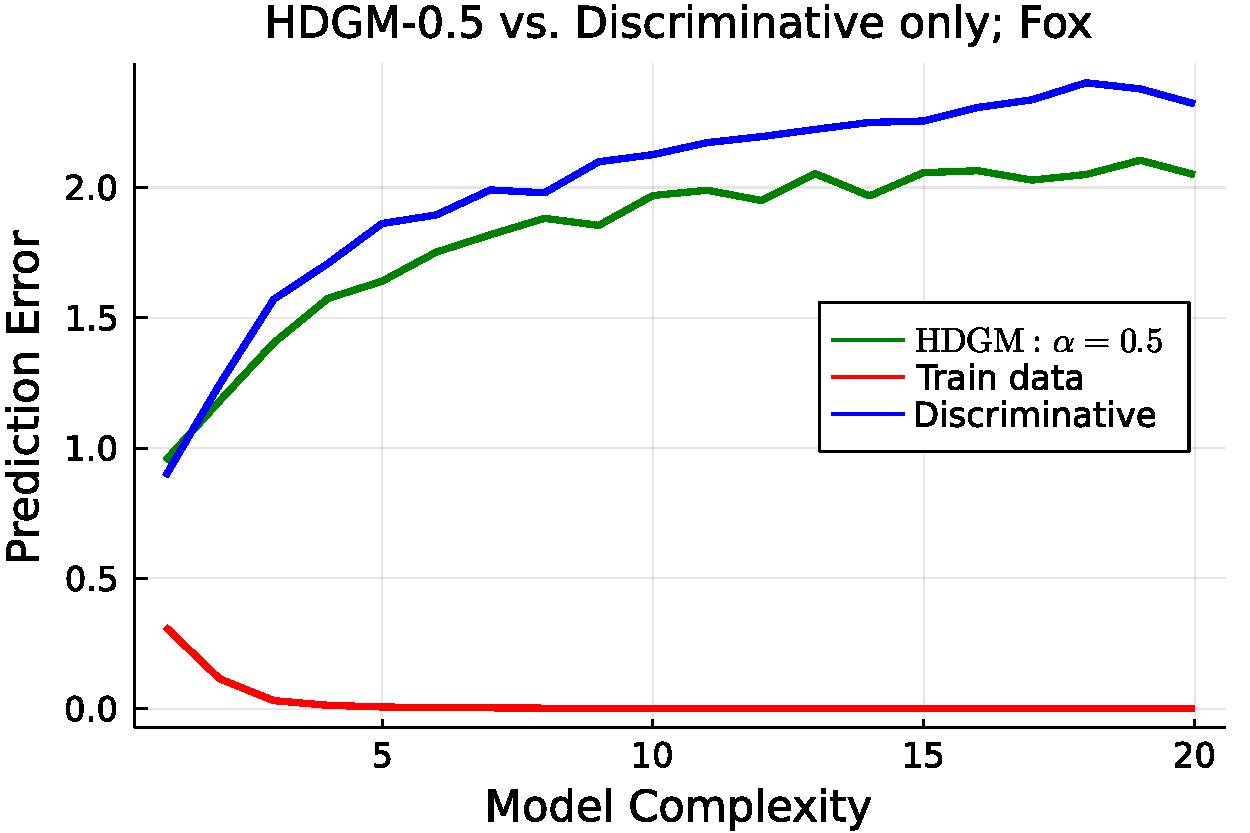
\includegraphics[width=8.2cm]{plots/Images/supervisedvsHDGM0_5_Fox.pdf} }}%
	\subfloat[HDGM: $\alpha=0.5$ vs Discriminative; Tiger.]
	{{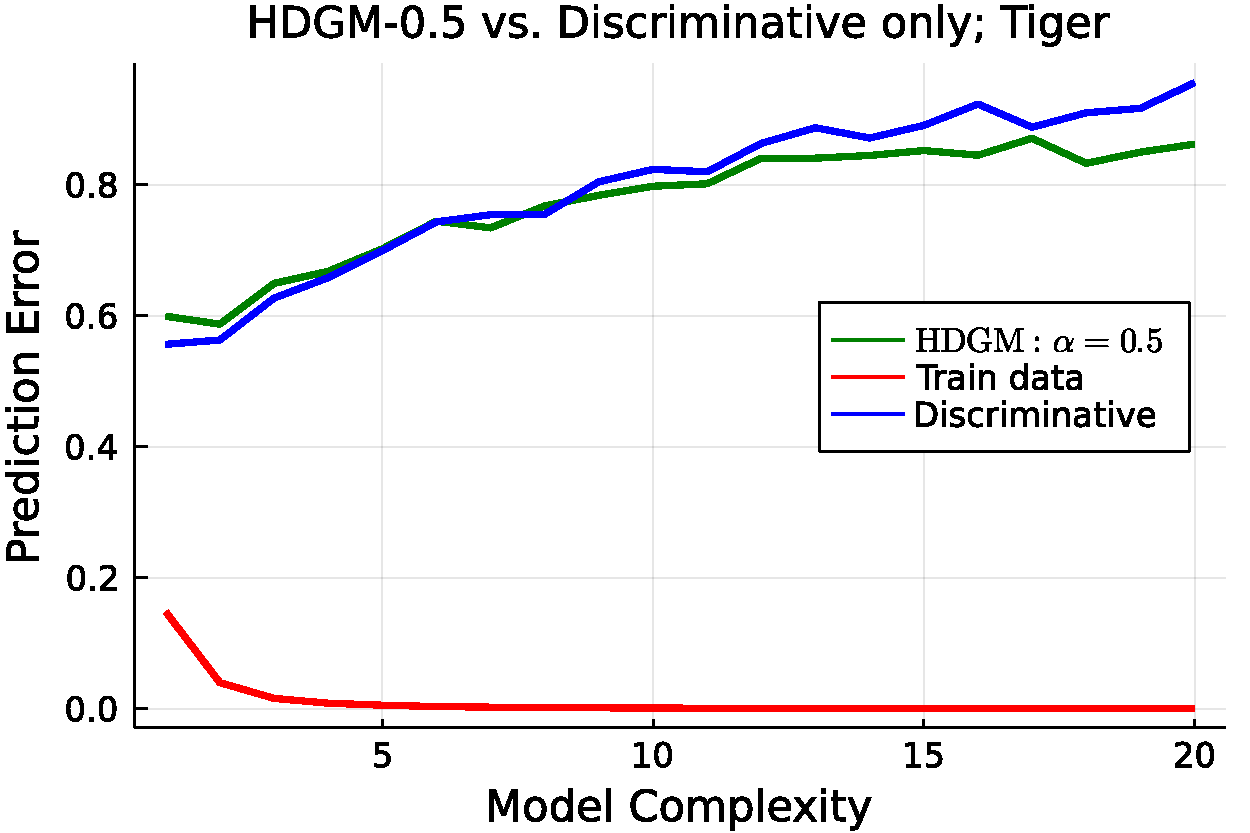
\includegraphics[width=8.2cm]{plots/Images/supervisedvsHDGM0_5_Tiger.pdf} }}
\caption{Comparison of the prediction error $\widehat{\mathrm{Err}}(z)$ for HDGM $\alpha=0.5$ and only the discriminative part. }%
	\label{fig:resultsHDGMz}%
\end{figure}
